% RMIT University School of CS&IT
% Minor thesis template
% S.M.M. (Saied) Tahaghoghi, 2004

\documentclass[11pt,twoside]{report}
\usepackage{a4wide,caption,epsfig,fancyheadings,url}
\usepackage{graphicx}
\graphicspath{ {./Figs/} }
\setcounter{secnumdepth}{3}

% Place the correct values here
%Set to the original submission date when submitted amended thesis
\newcommand{\SubmissionDate}{\today}
\newcommand{\student}{Tyler Saxton}
\newcommand{\supervisor}{Dhirendra Singh}
\newcommand{\topic}{Mapping suburban bicycle lanes using street scene images and deep learning}
\newcommand{\school}{School of Computer Science and Information Technology}
\newcommand{\program}{Masters of Data Science}
\newcommand{\institution}{Royal Melbourne Institute of Technology}

% Use the remark command to highlight text for discussion
\newcommand{\remark}[1]{{\bf \em [\marginpar{$\Leftarrow$}#1]}}

\renewcommand{\leftmark}{\student}
\renewcommand{\rightmark}{\topic}
\renewcommand{\headrulewidth}{0pt}
\setlength{\parindent}{0pt}
\setlength{\parskip}{1.5ex plus 0.3ex}

% This is the line spacing - set to 2 for draft submission to
% supervisor, 1.3 for the final submission
\renewcommand{\baselinestretch}{1.3}

\renewcommand{\captionfont}{\it}
\raggedbottom

\begin{document}

%%%%%%%%%%%%%%%%%%%%%%%%%%%%%%%%%%%%%%%%%%%%%%%%%%%%%%%%%%%%%%%%%%%%%%
\title{{\Large\bf \topic}}
\author{
A minor thesis submitted in partial fulfilment of the requirements for the degree of
\\\program\\*[10mm]
%\epsfig{figure=Figs/rmit-coa.epsf,width=5cm}
\\\student
\\\school
\\Science, Engineering, and Technology Portfolio,
\\\institution
\\Melbourne, Victoria, Australia
}
\maketitle
\thispagestyle{empty}


%%%%%%%%%%%%%%%%%%%%%%%%%%%%%%%%%%%%%%%%%%%%%%%%%%%%%%%%%%%%%%%%%%%%%%
\chapter*{Declaration}

This thesis contains work that has not been submitted previously, in
whole or in part, for any other academic award and is solely my
original research, except where acknowledged.

This work has been carried out since March 2021, under the
supervision of {\supervisor}.

\paragraph{}
\vspace{5cm}\noindent \\\student \\
\school\\
\institution\\
\SubmissionDate

\pagenumbering{roman}

%%%%%%%%%%%%%%%%%%%%%%%%%%%%%%%%%%%%%%%%%%%%%%%%%%%%%%%%%%%%%%%%%%%%%%
\chapter*{Acknowledgements}

First and foremost, I would like to thank Dr. Dhirendra Singh for inspiring this research and supervising me throughout the year.  I also greatly appreciate the input provided by Dr. Ron van Schyndel and the ``Research Methods'' class of Semester 1 2021, as I worked to develop a detailed research proposal. \\

To Dr. Sophie Bittinger, Dr. Logan Bittinger, Laura Pritchard, and Dr. Curtis Saxton, thank you for your encouragement, and your assistance with the editing process.



%%%%%%%%%%%%%%%%%%%%%%%%%%%%%%%%%%%%%%%%%%%%%%%%%%%%%%%%%%%%%%%%%%%%%%
\chapter*{To-Do}

\begin{itemize}
\item{Revisit abstract to update the scope of results based on any other suburbs tested}
\item{Repetitive language between Summary and Abstract ``this thesis presents''}
\item{I'm sure I had a better paper on road boundary detection, find it!}
\item{Thesis examples have ``Contribution'' and ``Organisation'' sections}
\item{Insert example GSV detection image}
\end{itemize}

%%%%%%%%%%%%%%%%%%%%%%%%%%%%%%%%%%%%%%%%%%%%%%%%%%%%%%%%%%%%%%%%%%%%%%
\chapter*{Summary}

Many policy makers around the world wish to encourage cycling, for health, environmental, and economic reasons.  One significant way they can do this is by providing appropriate infrastructure, including formal on-road bicycle lanes.  It is important for policy makers to have access to accurate information about the existing bicycle network, in order to plan and prioritise upgrades.  Cyclists also benefit when good maps of the bicycle network are available to help them to plan their routes.  This thesis presents an approach to constructing a map of all bicycle lanes within a local area, based on computer analysis of street scene  images sourced from Google Street View or ``dash cam'' footage.

% https://tex.stackexchange.com/questions/131460/remove-pagebreak-after-a-chapter-only-for-one-chapter
\begingroup
\renewcommand{\cleardoublepage}{}
\renewcommand{\clearpage}{}
\chapter*{Abstract}
\endgroup

On-road bicycle lanes improve safety for cyclists, and encourage participation in cycling for active transport and recreation.  With many local authorities responsible for the infrastructure, official maps and datasets of bicycle lanes may be out-of-date and incomplete.  Even ``crowdsourced'' databases may have significant gaps, especially outside popular metropolitan areas.  This thesis presents a method to create a map of bicycle lanes in a local area by taking sample street scene images from each road,  and then applying a deep learning model that has been trained to recognise bicycle lane symbols.  The list of coordinates where bicycle  lanes were detected is then correlated to geospatial data about the road network to record bicycle lane routes.  The method was applied to successfully build a map for a local area in the outer suburbs of Melbourne.  It was able to identify bicycle lanes not previously recorded in the official State government dataset, OpenStreetMap, or the ``biking'' layer of Google Maps.

%%%%%%%%%%%%%%%%%%%%%%%%%%%%%%%%%%%%%%%%%%%%%%%%%%%%%%%%%%%%%%%%%%%%%%

\tableofcontents
\listoffigures
\listoftables


%%%%%%%%%%%%%%%%%%%%%%%%%%%%%%%%%%%%%%%%%%%%%%%%%%%%%%%%%%%%%%%%%%%%%%
\chapter{Introduction}
\pagenumbering{arabic}

\remark{Criteria 15: clear research questions/aims/hypotheses}

\remark{Criteria 15: background knowledge}

The benefits of ``active transport'', such as walking and cycling, have been well documented in previous studies.  Participants' health may improve due to their increased physical activity.  There are environmental benefits due to reduced emissions and pollution.  And there are economic benefits, including a reduced burden on the health system, and reduced transportation costs for participants \cite{LEE2012219} \cite{RABL2012121}.

Federal and State government policy makers in Australia therefore wish to encourage cycling \cite{federal_policy_2019} \cite{state_policy_2020}.  However, the share of cycling for trips to work in Melbourne is only 1.5\% \cite{melbactive}.  For many commuters, a perceived lack of safety of cycling is a major barrier to adoption.  Other significant factors are the availability of shared bicycle schemes and storage facilities, and the risk of theft \cite{WILSON2018234}.  Cycling infrastructure has a significant impact on real and perceived cyclist safety, and this research project will focus on that issue.  Important safety factors include the presence and width of a bicycle lane, the presence of on-street parking, downhill and uphill grades, and the quality of the road surface \cite{BIKESAFETY} \cite{Teschke2012}.  A comprehensive dataset of cycling infrastructure would help policy makers identify and prioritize areas in need of improvement to safety.

In Victoria, Australia, the State government publishes a ``Principal Bicycle Network'' dataset to assist with planning \cite{PrincipalBicycleNetwork}, however it does not appear to be up-to-date.  Individual Local Government Areas may produce their own maps of bicycle routes, but availability is inconsistent \cite{vicroads_maps}.

The aim of this research project was to investigate whether it is possible to construct a dataset or map of bicycle lanes in a local area, by collecting street scene images at known coordinates, and then using a ``deep learning'' machine learning model to detect locations where bicycle lanes are found.  If a baseline map of bicycle lanes can be built in this way, then the process could be extended in future to gather information about other significant factors, such as how frequently the bicycle lane is obstructed by parked vehicles, or the presence of debris or damage to the road surface.

Google Street View has been chosen as a source of street scene image data due to its wide geographical coverage, and the accessibility of the data via a public API.  However, a significant limiting factor is that the Google Street View images for any given location might be several years out of date.  Therefore, the use of images collected from a ``dash cam'' was also explored.  A local government that is responsible for building and maintaining bicycle lanes could use dash cameras to gather its own images, at regular intervals, for more up-to-date data.

\section{Research Questions}
\begin{itemize}
\item{RQ1: Can a ``deep learning'' machine learning model be used to identify on-road bicycle lanes in street scene images sourced from Google Street View?}
\item{RQ2: Can the model then be used to detect and map bicycle lanes across all streets in a local area with Google Street View coverage?}
\item{RQ3: Can a similar process be applied to street scene images collected from dash camera video footage?}
\end{itemize}


%%%%%%%%%%%%%%%%%%%%%%%%%%%%%%%%%%%%%%%%%%%%%%%%%%%%%%%%%%%%%%%%%%%%%%
\chapter{Literature Review}

\remark{Criteria 15: literature review places research in context}

\remark{Criteria 15: background knowledge}

% ~~~~~~~~~~~~~~~~~~~~~~~~~~
\section{Motivation}

Prior research has clearly shown health, economic, and environmental benefits from active transport.  Lee et al., 2012 \cite{LEE2012219} analysed World Health Organization survey data from 2008, and showed that physical inactivity significantly increased the relative risk of coronary heart disease, type 2 diabetes, breast cancer, colon cancer, and all-cause mortality, across dozens of countries.  Rabl \& de Nazelle, 2012 \cite{RABL2012121} demonstrated that active transport by walking or cycling improves those relative risks for participants.  Moderate to vigorous cycling activity for 5 hours a week reduced the all-cause mortality relative risk by more than 30\%.  They estimated an economic gain from improved participant health and reduced pollution, offset slightly by the cost of cycling accidents.

In Australia, Federal and State governments are committed to the principle of supporting active transport through the provision of cycling infrastructure, declaring their commitment through public statements on their official websites \cite{federal_policy_2019} \cite{state_policy_2020}.  Many other governments around the world have adopted similar policies.

Taylor \& Thompson, 2019 \cite{melbactive} surveyed the use of active transport in Melbourne, to establish a baseline of current commuter behaviour.  They found that cycling only accounted for 1.5\% of trips to work in the area.  It could therefore be argued that there is room for improvement.

Schepers et al., 2015 \cite{SCHEPERS2015460} produced a summary of literature related to cycling infrastructure and how it can encourage active transport, resulting in the aforementioned benefits.  The paper found that providing cycling infrastructure that is perceived as being safer does encourage participation.  Other papers such as Wilson et al., 2018 \cite{WILSON2018234} agreed.

Other researchers have examined which factors affect the perceived and actual safety of cycling routes, in a variety of settings.

Klobucar \& Fricker, 2007 \cite{BIKESAFETY} surveyed a group of cyclists in Indiana, USA, asking them to ride a particular route and rate the safety of each road segment along the route, then asking them to review video footage of other routes and rate the safety of those routes, too.  A regression model was created to predict the cyclists' likely safety ratings for other routes.  The creation of the model led to a list of road segment characteristics that were apparently most influential in the area.

Tescheke et al., 2012 \cite{Teschke2012} surveyed patients who attended hospital emergency rooms in Toronto and Vancouver in Canada, due to their involvement in a cycling accident.  Details of the circumstances of each accident were gathered, along with the outcomes.  The data was analysed to determine which factors increased (or decreased) the relative odds of a cyclist being involved in an accident.

Malik et al., 2021 \cite{Malik2021} modelled cyclist safety in Tyne and Wear County in north-east England, a more rural setting.

The factors that contribute to cyclist safety vary by locality.  For example, cyclists in one city might be concerned by the hazard of tram tracks, whereas this might not be a relevant concern in another city, or a less built-up area.  The common themes among the aforementioned papers were:
\begin{itemize}
\item{Presence and type of bicycle lane (dedicated, paved shoulder, none)}
\item{Width of bicycle lane}
\item{Presence of on-street parking}
\item{Downhill or uphill grades}
\item{Volume, speed, and vehicle type profile of motor vehicle traffic}
\item{Quality of road surface (including drainage, tram tracks, etc.)}
\item{Lighting}
\item{Construction Work}
\end{itemize}
Most of these factors can be influenced by infrastructure and road design.  Therefore, it would be valuable to quantify as many of these factors as possible in a dataset, to assist policy makers in deciding what changes ought to be made, and where, to provide a safer network of cycling infrastructure.

% ~~~~~~~~~~~~~~~~~~~~~~~~~~
\section{Applications of Machine Learning}

``Deep Learning'' is a paradigm by which computational models can be constructed to tackle many problems, including visual object recognition.  A Deep Learning model can be trained to perform visual object recognition tasks by supplying it with a ``training'' dataset of images where the objects it must recognise have been pre-labelled.  During training, the model processes its training dataset over and over again, and with each iteration the weights in its multi-layer neural network are refined through the use of a ``backpropagation'' algorithm \cite{deeplearning}.  With a sufficient number of training ``epochs'', the model hopefully develops the ability to detect where the objects of interest appear in each image, to an acceptable level of performance.

Tensorflow \cite{TENSORFLOW2016A} \cite{TENSORFLOW2016B} and PyTorch \cite{pytorch} are two dominant frameworks for building, training, evaluating, and applying Deep Learning models.  Within these frameworks, researchers have progressively developed new models for visual object recognition, typically with a focus on either improving the accuracy of the results, increasing speed to allow ``real time'' processing of video streams, or creating models that will work on low-cost hardware.  Significant Deep Learning models considered within this research project include:

\begin{itemize}
\item{Ren et al., 2015 \cite{REN2016} R-CNN}
\item{Liu et al., 2016 \cite{ssd} SSD}
\item{He et al., 2016 \cite{He_2016_CVPR} ResNet}
\item{Redmon et al., 2016 \cite{YOLOv1} YOLO (and subsequent variants)}
\item{Sandler et al., 2018 \cite{MobileNetV2} MobileNetV2}
\item{Duan et al, 2019 \cite{centernet} CenterNet}
\end{itemize}

The Tensorflow 2 Model Garden \cite{zoo} provides access to many of these models, pre-trained on the COCO 17 (``Microsoft COCO: Common Objects in Context'') dataset.  It therefore provides a convenient library of Deep Learning models that have already received a significant amount of training for the general problem of visual object recognition, and can be re-used to recognise new classes of objects through a process of ``transfer learning'' \cite{coco} \cite{transferlearning}.

Semantic image segmentation of street scene images is an important and active area of computer science research.  ``Deep Learning'' models that can understand sequences of images in real time are essential for self-driving vehicles or similar driver-assistance systems, so many papers have focussed on that area.  In order to train a Deep Learning model that specializes in understanding street scene images, a training dataset of street scene images is required.  Papers by Cordts et al., 2016 \cite{Cordts_2016_CVPR} and Zhou et al., 2019 \cite{ade20k} announced the publication of the ``Cityscapes'' and ``ade20k'' image datasets, respectively.  These datasets each contain many street scene images, with objects of interest labelled in a format suitable for training deep learning models to understand similar on-road scenarios.  Many papers have used these datasets in order to train new machine learning models.  Chen et al., 2018 \cite{DEEPLAB} is one example of a heavily-cited paper where ``CityScapes'' data has been used to train a ``real time'' model to understand street scene images.  Unfortunately, neither of the datasets has cycling infrastructure labelled.  The ``CityScapes'' dataset has labelled bicycle lanes under the ``sidewalks'' category.  This is useful to train a car not to drive there, but a cyclist might not be legally allowed to ride on a sidewalk designed for pedestrian traffic.  

In another branch of research, deep learning tools have been used to manage roadside infrastructure and assets.  Campbell et al., 2019 \cite{CAMPBELL2019101350} used an ``SSD MobileNet'' model to detect ``Stop'' and ``Give Way'' signs on the side of the road in Google Street View images, to help build a database of road sign assets.  An application called ``RectLabel'' was used to label 500 sample images for each type of sign.  Photogrammetry was used to estimate a location for each detected sign, based on the Google Street View camera's position and optical characteristics and the bounding box of the detected sign.  Zhang et al., 2018 \cite{s18082484} performed a similar exercise, detecting road-side utility poles using a ``ResNet'' model.

In Australia, the ``Supplement to Australian Standard AS 1742.9:2000'' sets out the official standards for how bicycle lanes must be constructed and marked.  Generally, a lane marking depicting a bicycle should be painted on the road inside the bicycle lane within 15 metres before and after each intersection, and at 200m intervals \cite{standards}.  Therefore, a Deep Learning model could be trained to detect these markings, similar to how Campbell et al., 2019 \cite{CAMPBELL2019101350} trained a model to detect road signs, and Zhang et al., 2018 \cite{s18082484} trained a model to detect utility poles, using pre-trained models from the TensorFlow 2 Model Garden \cite{zoo} as a starting point.

The use of satellite imagery and aerial photographs were also considered.  Li et al., 2016 \cite{ROADNETWORK} showed that a road network could be extracted from satellite imagery using a convolutional neural network (CNN), and this is particularly useful in rural areas where maps are not already available.  However the resolution of publicly available satellite image data would not be sufficient to identify a bicycle lane on a road, and it would not be able to distinguish a standard bicycle lane from a wide paved shoulder.  Satellite imagery may have a role to play in detecting off-street bicycle tracks in ``green'' parkland area, but it was decided to exclude off-street routes from the scope of this research.

Aerial photography may be useful, where it is available with sufficient detail.  However it would require a different data source for every jurisdiction.  Ning et al., 2021 \cite{NING2021} had success extracting sidewalks from local aerial photography using a ``YOLACT'' model.  Areas of uncertainty caused by tree cover were filled in using Google Street View images.  The model appeared to rely on a concrete sidewalk having a very different colour to the adjacent bitumen road.  The approach might not be able to distinguish bitumen bicycle lanes.  The road markings were not visible.

Aside from formal bicycle lanes, cyclist safety can also be improved by an informal wide paved shoulder, or by creating lanes that are wide enough to safely accommodate a vehicle passing a cyclist.  It may be possible to detect and map these arrangements by recognising lane markings and road boundaries.  A common method of detecting lane boundaries is through the combination of a Canny edge detector \cite{canny} and a Hough transformation \cite{hough}.  The OpenCV library provides a frequently used implementation \cite{opencv}.  Where the Canny-Hough approach struggles with a poorly defined road boundary or ``noise'' from roadside objects, a Deep Learning approach may help:  Mamidala et al., 2019 \cite{8929655} used a ``CNN'' model to detect the outer boundary of roads in Google Street View images.

During the literature review, one other paper was identified where the authors had applied Deep Learning techniques in the domain of cyclist safety:  Rita, 2020 \cite{rita_2020} used the ``MS Coco'' and ``CityScapes'' datasets to train ``YOLOv5'' and ``PSPNet101'' models to identify various classes of object (Bicycle, Car, Truck, Fire Hydrant, etc.) in Google Street View images of London.  A matrix of correlations between objects was calculated.  This was used to infer the circumstances where cyclists might feel the most safe.  For example, there was a high correlation between ``Person'' and ``Bicycle'' which ``suggests pedestrians and cyclists feel safe occupying the same space''.  This is a complimentary approach that might serve to help policy makers to identify where there is demand for better infrastructure.


% ~~~~~~~~~~~~~~~~~~~~~~~~~~
\section{Available Cycling Infrastructure Datasets and Standards}

In Victoria, the State Government started publishing an official ``Principal Bicycle Network'' dataset on \url{data.gov.au} in 2020 \cite{PrincipalBicycleNetwork}.  It includes ``existing'' and ``planned'' bicycle routes.  There is a field to record the width of a bicycle lane to the nearest metre, but it is not always populated.  Many entries have been marked as last being ``validated'' in 2014, or not at all.  The dataset only covers formal bicycle lanes, so it excludes roads where the cyclist may ride on a less formal paved shoulder.  During the course of the research, it was found that some existing bicycle lanes are still marked as ``planned'', or not listed at all, and in some country areas the routes appeared to be paved shoulders rather than standard bicycle routes.

``OpenStreetMap'' \cite{OPENSTREETMAP} is a source of crowd-sourced map data.  It provides detailed information aabout roads with and without bicycle lanes.  It supports ``cycleway'' tags where contributors can mark not just where a bicycle lane is, but its attributes, such as whether it is shared with public transport, whether there is a specially marked area for cyclists to stop at intersections, and how wide the bicycle lane is.  Given that the data is crowd-sourced, the quality and availability of the data may vary by location.

``Google Maps'' provides a ``bicycle layer''.  This includes off-street bicycle paths and on-street bicycle lanes.  It only gives a ``yes'' or ``no'' opinion about whether a route is especially suited to bicycles, with no further information provided.  But that may be of assistance in scouting locations to use in a training dataset of Google Street View images.

Other services such as ``Strava'' and ``Trailforks.com'' hold data that cyclists have recorded about their rides.  These may be useful to assess the popularity of routes, and perhaps infer where upgrades would be welcomed, or where there might be an existing route that should be checked and added to a dataset.


%%%%%%%%%%%%%%%%%%%%%%%%%%%%%%%%%%%%%%%%%%%%%%%%%%%%%%%%%%%%%%%%%%%%%%
\chapter{Methods}

\remark{Criteria 15: clear and accurate description of methods}

\remark{Criteria 15: sufficient detail to allow reproduction of results}

\remark{Criteria 15: awareness and critical evaluation of alternatives}

This section describes the methodology that was used to address each of the research questions.

\remark{Comment on where to find github repository of code, where to find original source dashcam videos and GSV training image lists}

For detailed instructions on how to reproduce the results using the source code and data provided, please refer to the accompanying appendices.

% ~~~~~~~~~~~~~~~~~~~~~~~~~~
\section{RQ1: Training a model to identify bicycle lanes in Google Street View images}
\label{s:rq1}

A review of the relevant Australian standards for bicycle lanes \cite{standards}, combined with local knowledge, suggested that the best way to search for bicycle lanes in street scene images would be to train a model to search for the bicycle lane markings that are painted on the road surface.  See figure \ref{fig:symbol}.  This marking is universal across all standard bicycle lanes in Australia, and can distinguish a bicycle lane from other types of road segment.  The symbol may appear sometimes appear on a green surface, and occasionally it may be partially occluded due to limited space or wear and tear.  Similar symbols exist in many other jurisdictions outside Australia.

\begin{figure}[h]
\centering
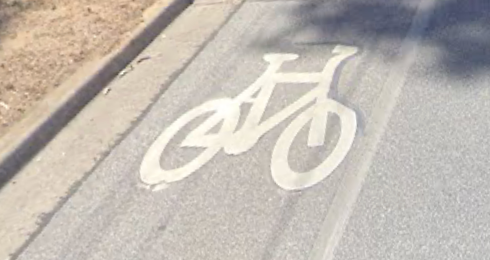
\includegraphics{f001_symbol.png}
\caption{Example bicycle lane marking.  Source: Google Street View, Oct 2019}
\label{fig:symbol}
\end{figure}

Therefore, in order to identify bicycle lanes in Google Street View images, it was necessary to first create a dataset of labelled images for training and validation, and then use it to train and evaluate Deep Learning models, using pre-trained models from the ``TensorFlow 2 Model Garden'' and transfer learning.

\subsection{Gathering a training dataset of Google Street View images}

A collection of Google Street View images containing bicycle lane markings was required, to train the Deep Learning models.  The relevant Australian standards specify that these markings should appear within 15m of each intersection \cite{standards}.  Therefore, intersections along known bicycle lane routes were the most likely locations to search for example images.

Campbell et al., 2019 \cite{CAMPBELL2019101350} found success training a Deep Learning model to recognise ``Stop'' and ``Give Way'' signs with 500 example images of each.  Therefore, an initial dataset of 500 bicycle lane marking images was required, with an option to gather more images if necessary.

A tool was required to efficiently gather sample images from Google Street View for intersections along known bike paths, and record which images contained the required markings.  These images could then be labelled using another tool, to record the precise bounding box around each bicycle lane marking in the images.

\subsubsection{Identifying candidate intersections to sample}

The two candidate sources of information about ``known'' bicycle lane routes that were considered were the ``Principal Bicycle Network'' dataset \cite{PrincipalBicycleNetwork} and XML extracts from the OpenStreetMap database \cite{OPENSTREETMAP}.  The Principal Bicycle Network dataset was used to identify candidate intersections due to its age:  If it was last updated several years ago, then there was less risk that an intersection being sampled would be missing bicycle lane markings in the Google Street View images due to the age of the available Google Street View data.  However, the OpenStreetMap approach has the advantage that it would work for other jurisdictions, and it proved to be less complex.

Tools were created to generate candidate intersection lists for both approaches.  Instructions on how to use them are documented in Appendix \ref{a:sample_pbn} and Appendix \ref{a:sample_osm}.

Working from an XML extract of the OpenStreetMap database is the simplest approach.  Data can be downloaded for an individual country via \url{https://download.geofabik.de} and then sliced into a smaller area, if necessary, using the ``osmium'' command line tool from \url{https://osmcode.org/osmium-tool/}.  Once downloaded, the XML contains ``ways'', which represent road segments, and ``nodes'', which represent strings of coordinates that make up the ``ways''.  If a ``way'' contains a ``cycleway'' tag, then it has a bicycle lane.  If a ``node'' is included in multiple ``ways'' then it is an intersection.  So the process is to identify ``ways'' with a ``cycleway'' tag, and then search the list of ``nodes'' in that way to see which ones are shared with any other ``way'' with a different name.

Working from the Principal Bicycle Network dataset is more complicated, and it still requires an XML extract of OpenStreetMap data to identify the intersections.  The Principal Bicycle Network dataset contains start and end coordinates for each segment of road where there ss an existing bicycle lane.  But it does not consistently include the name of the road, and it never included the town or suburb, nor any information about intersections.  To solve this problem, the following approach was taken:

\begin{enumerate}
\item{For each co-ordinate in the Principal Bicycle Network dataset, use a local ``Nominatim'' server instance to determine the name of the road and the town or suburb, via a ``reverse-geocoding'' operation.}
\item{For each named road and town or suburb in the reverse-geocoded dataset, use an XML extract of OpenStreetMap data for the area to identify intersecting roads.  Use a bounding box around the original route coordinates in order to eliminate false intersections for roads with the same name in a different town.}	
\end{enumerate}

A local instance of Nominatim was installed because the terms of use for public Nominatim server instances actively discourage bulk operations.  It was set up on a local machine as per Appendix \ref{a:computer} according to the official instructions \cite{nominatim_install}.

Once intersections were identified from the OpenStreetMap data, it proved to be helpful to also calculate an approximate heading along the bicycle lane route at each intersection, to ensure that Google Street View images could be requested with the camera facing in a sensible direction.  The heading from one point to the next can be calculated using the Python "geographiclib" library.  Therefore the heading at the intersection was calculated to be the average of the heading from the previous ``node'' on the ``way'' to the intersection node and the heading from the intersection node to the next node.

\subsubsection{Downloading sample Google Street View images for the training dataset}
\label{s:sample}

Google provides an API for downloading Google Street View images of up to 640x640 pixels, at a cost of \$7.00 USD per 1,000 images up to the first 100,000, discounted to \$5.60 USD per 1,000 images from 100,001 to 500,000, with further volume discounts negotiated with their sales team beyond that. \cite{gsv_billing}.  The ``\texttt{google\char`_streetview}'' library was used to facilitate access to this API from Python code.  In order to minimise costs, whenever an image was downloaded via the API, a copy of the image and its associated metadata was cached locally, so that additional costs would not be incurred if a request was made for the same image at a later date.

The API allows images to be requested for a location (latitude/longitude) with a desired heading, field-of-view angle, and camera angle relative to the ``horizon''.  A Jupyter Notebook was created to:

\begin{enumerate}
	\item{Select a sample location and heading from a CSV of candidate intersections.}
	\item{Download four Google Street View images at 0, 90, 180, and 270 degrees relative to the desired heading, with a 90 degree field of view for each image, and the camera angled 30 degrees towards the ground to focus on any nearby road markings.}
	\item{Allow the operator to quickly record which of the four images they see a bicycle lane marking in, so that it can be saved to a list of images to be labelled and included in the training dataset.}
	\item{Repeat.}
\end{enumerate}

It was found that the best location to look for a bicycle lane marking was not always right in the middle of an intersection, especially for large intersections.  Therefore, the option was added to allow the operator to ``browse'' a desired number of metres before or after the intersection, along the route heading, to find a good image.  If a bicycle lane marking appeared at the intersection, typically it could be found within 20-30m.

Generally, an image was accepted for inclusion in the training dataset if the bicycle lane marking was close and clear enough to be unambiguous without taking cues from the overall scene context.  The shape of the bicycle had to be visible.  If the symbol was so far away that it looked like a white blob on the road, and it could only be understood to be a bicycle lane marking by looking at how it was placed relative lane markings, then the image was not included, though the operator had the option of moving the camera close to it for a better look in a different image.

The Jupyter Notebook allowed multiple candidate intersections to be assessed per minute, and an initial set of 500 images was collected over the course of approximately 4 hours.

Please see Appendix \ref{a:download_gsv} for detailed instructions on how to use the supplied Jupyter Notebook to download Google Street View images for sample intersections, and flag matching images for inclusion in the labelled training dataset.

\subsubsection{Labelling the training dataset}
\label{s:label}

Once a suitable number of Google Street View images containing bicycle lane markings were collected, they were copied to a folder and then labelled using the open-source tool "labelImg" \cite{labelImg}.  Please refer to the tool's official documentation for installation and usage instructions.  The output of the tool was an XML file corresponding to the each original image file in the folder, in a format that could be understood by TensorFlow 2 training tools and scripts.

\subsection{Training and evaluating candidate models from the TensorFlow 2 Model Garden}

Training and evaluation of candidate models was conducted on a local computer that was already available, as described in Appendix \ref{a:computer}.  This task could also be performed on cloud-based infrastructure such as Google Collab, if required.  For general directions on how to set up a local computer to enable TensorFlow machine learning that takes advantage of GPU acceleration, please see Appendix \ref{a:setupenv}, for find the latest tutorials and guides online.

The training dataset that was collected in section \ref{s:sample} and labelled in section \ref{s:label} was randomly split into ``training'' and ``testing'' datasets according to an 80:20 ratio, using a ``bash'' shell script.

A Jupyter notebook was used to set up the experiment, by transforming the labelled image datasets into TensorFlow records, downloading and configuring a pre-trained model from the TensorFlow 2 Model Garden, and creating scripts to train and evaluate the model.

During the training process, the TensorFlow training script showed the ``loss'' performance after every 100 epochs, and the performance gradually improved as more training was conducted over the dataset.  Every few thousand epochs, the training was paused so that the model's performance could be evaluated against the withheld ``test'' datasets.  When training reached the point that any further epochs yielded greatly diminished returns, the training for the model was terminated, and it was compared to other candidate models.  As part of the evaluation process, image files were output containing the original image plus an overlay where the bounding boxes and ``confidence'' score of any detections were drawn.  These were inspected by quickly browsing through the images to confirm that the bicycle lane markings were being accurately located within each image, and any false positives or false negatives were understood.  An output CSV file was also created as part of the process, to record the coordinates and other location details of each image where a bicycle lane marking was detected.

Multiple pre-trained models from the TensorFlow 2 Model Garden were trialled, with selections guided by their published ``Speed'' and ``COCO mAP'' (mean Average Precision) metrics.  The process of building a map of bicycle lanes for an area can be considered a ``batch'' process, with no fixed time constraints, therefore Mean Average Precision was prioritized over speed.

Please refer to Appendix \ref{a:tensorflow_training} for detailed instructions on how to reproduce the training process.

% ~~~~~~~~~~~~~~~~~~~~~~~~~~
\section{RQ2: Building a map of bicycle lane routes from Google Street View images in an area}
\label{s:rq2}

In section \ref{s:rq1}, a model was trained to detect bicycle lane markings in a single street view image.  To generate a map or dataset of bicycle lanes in an area, the first step is to determine a list of locations for which Google Street View images should be downloaded and processed by the model.  A batch process is then used to process each image and record whether a bicycle lane marker was found.  Finally, the list of sample locations where there was a ``hit'' must be correlated to geospatial data about the road network to infer and draw routes on a map.

\subsection{Sampling strategy for Google Street View images}
\label{s:rq2a}

In section \ref{s:sample}, it was noted that Google currently advertises a minimum cost of \$7.00 USD per 1,000 Google Street View images, and that the most likely place to find a bicycle lane marker is in the area immediately surrounding an intersection.  It was also found that the Google Street View API would only return distinct images every 10 metres.  Two sampling strategies were considered:
\begin{itemize}
\item{Generating a list of sample points every 10 metres along every street in the area.}
\item{Generating a list of sample points within a configurable distance of each intersection in the area, at 10 metre intervals.	}
\end{itemize}

Depending on the density of intersections in an area, limiting the samples to the immediate area around intersections could result in a significant cost reduction.  The ``intersection'' strategy was chosen, with the option to switch to full 10 metre sampling strategy if the results showed that too many bicycle lanes were being missed, that might otherwise have been detected with more samples.

An OpenStreetMap XML extract file for the area was loaded into memory and used to iterate over all streets and intersections in the area, resulting in a CSV batch file of sample locations to be downloaded from Google Street View and processed by the model.  The size of the batch file was inspected to assess potential cost before proceeding with the download from Google Street View.

When loading and interpreting the OpenStreetMap XML extracts, it was important to understand that while a ``way'' object in the data typically represents a road segment, it may also represent the boundary of a reserve, a natural feature such as a coastline or creek, or a walking trail.  To avoid unnecessary requests to the Google Street View API for off-street locations, it was necessary to inspect the tags associated with each ``way'' to isolate actual road segments.

The resulting sample location CSV file included not just the coordinates of each point, but the OpenStreetMap ``way'' and ``node'' IDs that the sample came from, any offset (in metres) from the original ``node'' coordinates, and descriptive fields such as the street or road name to help with traceability.

Please see Appendix \ref{a:sample_area1} for detailed instructions on how to operate the tool that was used to generate a list of sample locations.

\subsection{Batch processing of Google Street View images}
\label{s:rq2b}

Once sample locations have been selected, the first stage of the batch process works through the list, downloading any Google Street View images that have not already been cached locally.  The second stage calls the detection model to process each image.  If one or more bicycle lane markings are detected in an image, a copy of the image is saved to a folder of ``hits'', with the bounding box and confidence score included in the image to show where the detection was found.  A record is also inserted into a CSV file of detection locations.  If no bicycle lane marking is found in the image, a copy is instead placed in a separate ``miss'' folder.  Partitioning the ``hits'' and ``misses'' into separate folders allows the operator to quickly browse the images to check for any false positives or false negatives.

\remark{FIGURE: detection image for GSV}

Please see Appendix \ref{a:gsv_batch} for detailed instructions on how to operate the tools to download and cache Google Street View images for a list of sample locations, and process them with the model.

\subsection{Converting detection points into bicycle lane routes on a map}
\label{s:rq2c}

The result of the previous batch process in section \ref{s:rq2b} is a list of locations where a bicycle lane marking was found.  The next step is to convert these detection points into contiguous routes that can be drawn as lines on a map.  Google Street View image samples were taken 0, 90, 180, and 270 degrees from the assumed heading at each point, to provide to provide 360 degree coverage.  This allows detection of bicycle lane markings not just in the the forward and rear views, but also close along side the camera vehicle, to improve the chances that an image will be found where the marking is clearly visible.  The detection model has been trained to detect markings in any orientation, and many of the samples will be taken at intersections.  Therefore, when drawing routes, proper consideration must be made about whether a detection belongs to the route being inspected, or an intersecting street.

Routes were inferred from the individual detection points based on the assumption that if markings were detected at two or more consecutive intersections along a street, there is a bicycle lane between them.  An option was given to allow for one or more missed detections at intersections before assuming that the route has been interrupted.

A continuous road may be divided up into multiple ``way'' segments in the OpenStreetMap data if any of their characteristics change from one segment to the next, such as the speed limit.  Therefore before inferring bicycle lane routes along a road from the detection points, it was necessary to link the ``way'' segments back up into a single chain.

Each inferred route was written to a .geojson file as a ``LineString Feature'' following the original co-ordinates of all ``nodes'' in the original OpenStreetMap data, from start to finish.

\subsection{Comparing results to other data sources}

Once a .geojson file has been produced with the detected bicycle lane routes, aligned to the co-ordinates of the road network in the OpenStreetMap XML extract, it can be drawn on a map in a Jupyter Notebook using the ``ipyleaflet'' library.

The total length of all routes in a .geojson file can be calculated by using the ``geographiclib'' library to calculate the distance between each pair of points along the route.

The original OpenStreetMap XML extract can be used to generate an equivalent .geojson file of bicycle lane routes in the area according to OpenStreetMap.  The data is filtered down to ``ways'' that are roads that have a ``cycleway'' related tag, and then a ``LineString Feature'' is written to an output .geojson for each cycleway.

The detected .geojson file and the OpenStreetMap-derived .geojson file can be drawn on maps side-by-side for visual comparison, and the differences can be measured at a high level by comparing the total length of the routes in each file.

To drill down further into the detail of the differences, multiple .geojson files were created:

\begin{enumerate}
\item{A .geojson file with all detected bicycle lanes}
\item{A .geojson file where a bicycle lane was detected that was not recorded in OpenStreetMap}
\item{A .geojson file where a bicycle lane was recorded in OpenStreetMap but not detected}
\item{A .geojson file where both the detection model and OpenStreetMap agree that there is a bicycle lane}	
\end{enumerate}

Items 2-4 can be drawn as layers on a single map, each with their own color, to highlight where the bicycle lanes are, and where they disagree.  By measuring the distances in the file, we can quantify how much agreement there is between the two sources, and how many metres worth of bicycle lane routes are in one but not the other.

The Principal Bicycle Network dataset is available in .geojson format.  A quick visual comparison can be made by drawing it on a map side-by-side with the detected bicycle lanes .geojson file.  To quantify the differences, including a measurement of where the sources agree or disagree:

\begin{enumerate}
\item{For each point in the Principal Bicycle Network dataset .geojson file, find the closest point in the OpenStreetMap XML extract and its ``node'' ID.  Exclude any points outside the bounding box of the area.}
\item{Use the coordinates of the matching ``node'' from the OpenStreetMap data, instead of the original coordinates from the Principal Bicycle Network dataset, to ensure that the sources are ``aligned'' on a common understanding  of where the road network is.}
\item{Produce four output .geojson files to compare the ``aligned'' Principal Bicycle Network dataset to the detected bicycle lanes, following the same basic process that was used for the OpenStreetMap comparison.}
\end{enumerate}


% ~~~~~~~~~~~~~~~~~~~~~~~~~~
\section{RQ3: Applying the process to dash camera footage}
\label{s:rq3}

\remark{Choice of hardware}

\remark{Gathering data from dash cam}

\remark{Preliminary results without retraining}

\remark{Re-training model to include dash cam images}

\remark{Handling false positives and refining the training dataset}


% ~~~~~~~~~~~~~~~~~~~~~~~~~~
\section{Extension: Detecting and mapping paved shoulders}

\remark{Detecting lane markings and the next lane over}

\remark{Transforming lane marking data into routes}


%%%%%%%%%%%%%%%%%%%%%%%%%%%%%%%%%%%%%%%%%%%%%%%%%%%%%%%%%%%%%%%%%%%%%%
\chapter{Results and Discussion}

\remark{Criteria 40: clear and complete presentation of results}

\remark{Criteria 40: sufficient quantity of work}

\remark{Criteria 40: appropriate intellectual level}

\remark{Criteria 40: appropriate consideration of evidence in discussion}

\remark{Criteria 40: uncertainty/error analysis}

Discuss the limitations of GSV
- Time
- Bad luck with obstructions
- Position of camera
- Cost

Compare to use of dash camera
- More current

%%%%%%%%%%%%%%%%%%%%%%%%%%%%%%%%%%%%%%%%%%%%%%%%%%%%%%%%%%%%%%%%%%%%%%
\chapter{Conclusion}

\remark{Criteria 15: conclusions are supported by the observations/results/calculations}

\remark{Criteria 15: conclusions relate to the original research questions/aims/hypotheses}

%%%%%%%%%%%%%%%%%%%%%%%%%%%%%%%%%%%%%%%%%%%%%%%%%%%%%%%%%%%%%%%%%%%%%%
\appendix
\chapter{Computer Environment}
\label{a:environment}

Two computers were used

\section{Machine Learning workstation}
\label{a:computer}

xxx

\section{Nominatim server}
\label{a:nominatim}

xxx

\chapter{Identifying candidate intersections to sample based on cycleways in an OpenStreetMap XML extract}
\label{a:sample_osm}

xxx

\chapter{Identifying candidate intersections to sample based on existing bicycle lanes in the Principal Bicycle Network dataset}
\label{a:sample_pbn}

xxx

\chapter{Downloading and flagging sample Google Street View images for the training dataset}
\label{a:download_gsv}

xxx

\chapter{General directions on setting up a local TensorFlow 2 development environment}
\label{a:setupenv}

xxx

\chapter{Training and evaluating a Deep Learning model from the Tensorflow 2 Model Garden}
\label{a:tensorflow_training}

xxx

\chapter{Sampling Google Street View images from a local area}
\label{a:sample_area1}

xxx

\chapter{Batch processing of Google Street View images}
\label{a:gsv_batch}

xxx

\chapter{Constructing a map from Google Street View detections}
\label{a:gsv_map}

xxx

\chapter{Applying model to Dash Camera footage}
\label{a:apply_dashcam}

xxx

\chapter{Detecting paved shoulders from Dash Camera footage}
\label{a:lane_detection}

xxx

\cleardoublepage
\bibliographystyle{IEEEtran}
\bibliography{Bib/references.bib}
\end{document}
\end{document}
